\documentclass{article}
\usepackage{tikz}
\usepackage{verbatim} %commenting package
\usetikzlibrary{arrows}
\usetikzlibrary{calc,intersections,through,backgrounds}
\usetikzlibrary{automata}
\pagestyle{empty}
\begin{document}


% Define style for nodes
\tikzstyle{vertex}=[circle, draw, fill=black,
                        inner sep=0pt, minimum width=4pt]
%  Tutte's 8-cage

\begin{comment}
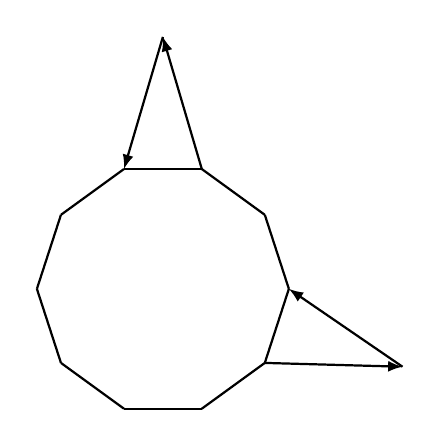
\begin{tikzpicture}[thick,scale=0.8]
    % The following path utilizes several useful tricks and features:
    % 1) The foreach statement is put inside a path, so all the edges
    %    will in fact be a the same path.
    % 2) The node construct is used to draw the nodes. Nodes are special
    %    in the way that they are drawn *after* the path is drawn. This
    %    is very useful in this case because the nodes will be drawn on
    %    top of the path and therefore hide all edge joins.
    % 3) Simple arithmetics can be used when specifying coordinates.
    
     \foreach  \x in {0,36,...,324}
    {
        \draw(\x:2) node {}  --  (\x-36:2);
      };
    
    \draw[->,>=latex]  (-36:2) node {} -- (-18:4);
    \draw[->,>=latex]  (-18:4) node {} -- (0:2);
    \draw[->,>=latex]  (2*36:2) node {} -- (90:4);
    \draw[->,>=latex]  (90:4) node {} -- (3*36:2);
\end{tikzpicture}\quad
\end{comment}

\begin{tikzpicture}

\tikzstyle{vertex}=[circle, draw, fill=black,
                        inner sep=0pt, minimum width=4pt]
                        
\node[vertex,label={0}](v0) at (1,0.5) {};
\node[vertex,label=below/:{1}](v1) at (0:2) {};
\node[vertex,label={n+1}](v2) at (15:4) {}; 
\node[vertex,label={2}](v3) at (30:2) {}; 

\node[circle, draw=black,scale=12] (a) at (0,0) {};
\node[circle, draw=white,label={\Huge $G$},scale=1] (a) at (0,-.5) {};

%\draw (0,0) circle (2);
\draw [->,>=latex,thick] (v1) -- (v2);
\draw [->,>=latex,thick] (v2) -- (v3);

% \draw [->,>=latex,thick] (v1) [out=10, in=-10] to  (v3);

\end{tikzpicture}

\end{document} 